\documentclass{article}
\usepackage[utf8x]{inputenc} % codifica scrittura
\usepackage[nochapters]{classicthesis} % nochapters
\usepackage[italian]{babel}
%\usepackage{inputenc}
\usepackage[T1]{fontenc} 
\usepackage[square,numbers]{natbib} 
\usepackage{amsmath, amsthm, amssymb, tikz}
\usetikzlibrary{snakes}
\newtheorem{definizione}{Definizione}  
\newtheorem{lemma}{Lemma}
\newtheorem{teorema}{Teorema}  
\newtheorem{proprieta}{Proprietà}  
\usepackage{titletoc}
\usepackage{verbatim}

\titlecontents{section}[3em]{}{\contentslabel{1em}}{}{\titlerule*[1.5pc]{.}\contentspage}
\titlecontents{subsection}[6em]{}{\contentslabel{2em}}{}{\titlerule*[1.5pc]{.}\contentspage}

\begin{document}

\title{\rmfamily\normalfont\spacedallcaps{Computer Aided Graphic
    Design course exercises}}

\author{\spacedlowsmallcaps{Massimo Nocentini}}
\date{} % no date

\maketitle


\begin{abstract}
  In questo lavoro ci proponiamo di studiare il risultato di
  impossibilità del consenso in un sistema totalmente asincrono,
  dimostrato da Michael J. Fischer, Nancy A. Lynch e Michael
  S. Paterson nel 1985.

  Nella nostra esposizione intendiamo riportare i principali risultati
  raggiunti dagli autori, integrando alcuni dettagli con brevi
  interventi che abbiamo sviluppato durante lo studio.

  Questo nostro elaborato è diviso in due macro sezioni: la prima ha
  un taglio più teorico e tratta la prova d'impossibilità; la
  seconda, invece, ha un taglio più implementativo e propone uno
  schema per risolvere il problema del consenso, aggiungendo alcune
  ipotesi.
\end{abstract}
       
\tableofcontents

\newpage

\section{Bezier curves from first exercise set}
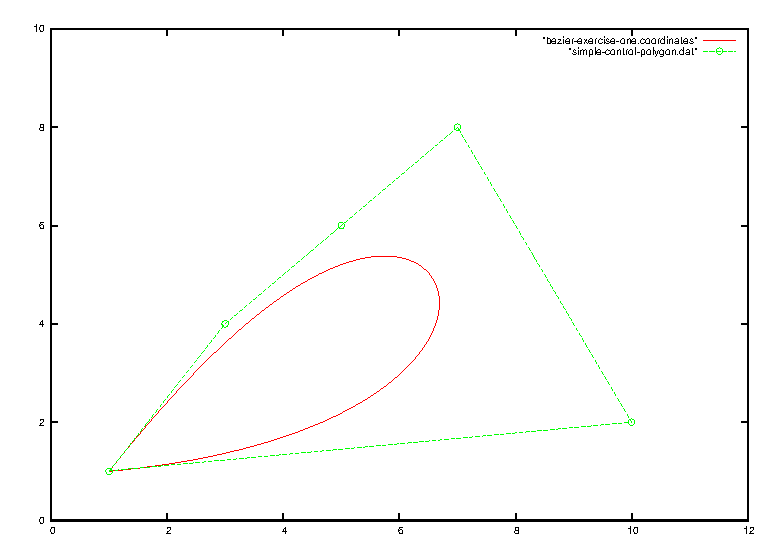
\includegraphics{bezier-deCasteljau-curves/exercise-one}
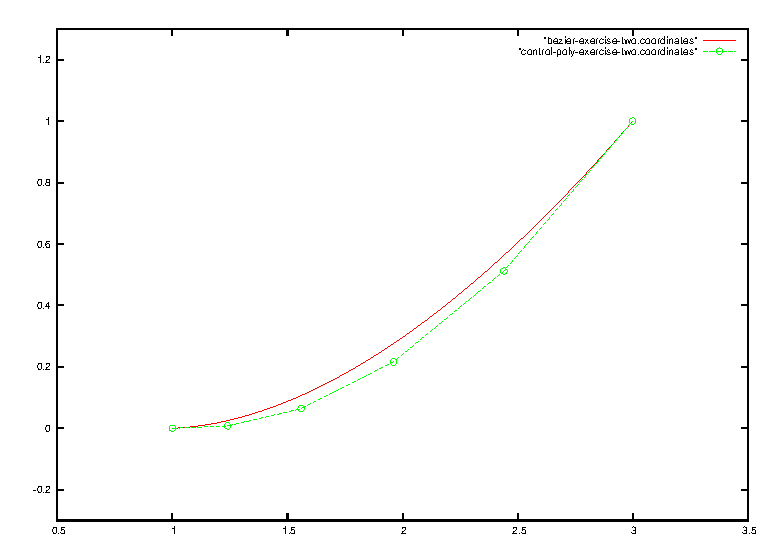
\includegraphics{bezier-deCasteljau-curves/exercise-two}
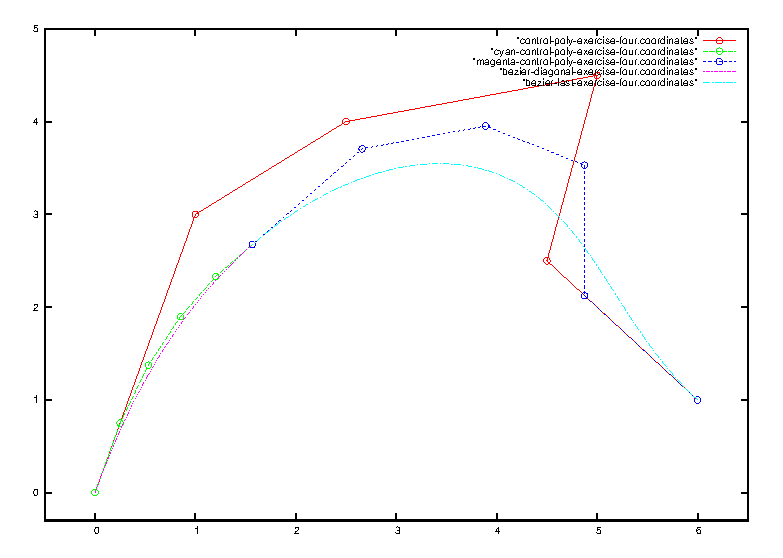
\includegraphics{bezier-deCasteljau-curves/exercise-four}
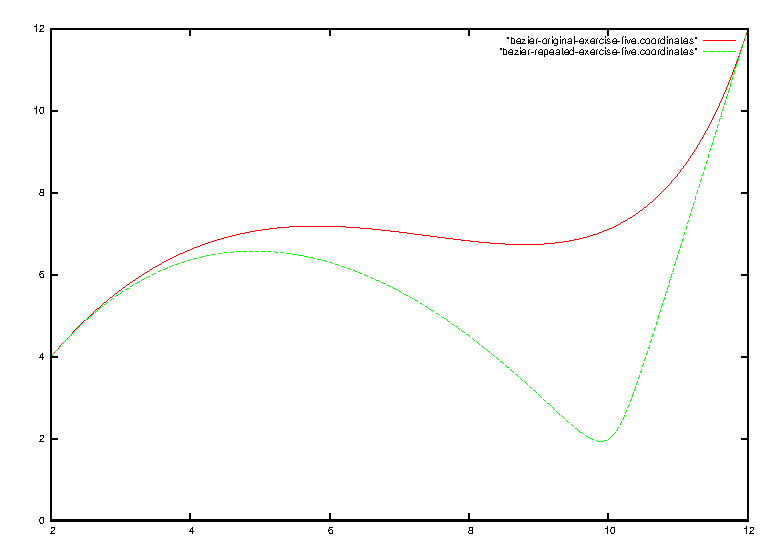
\includegraphics{bezier-deCasteljau-curves/exercise-five}
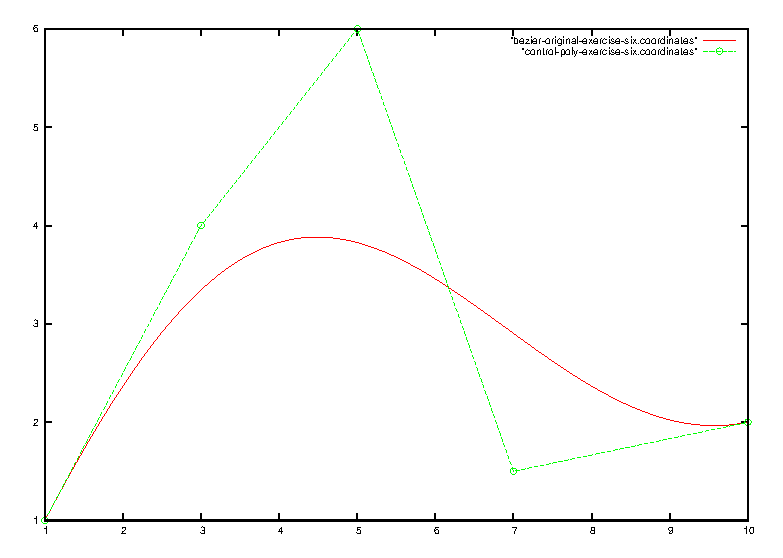
\includegraphics{bezier-deCasteljau-curves/exercise-six-original}
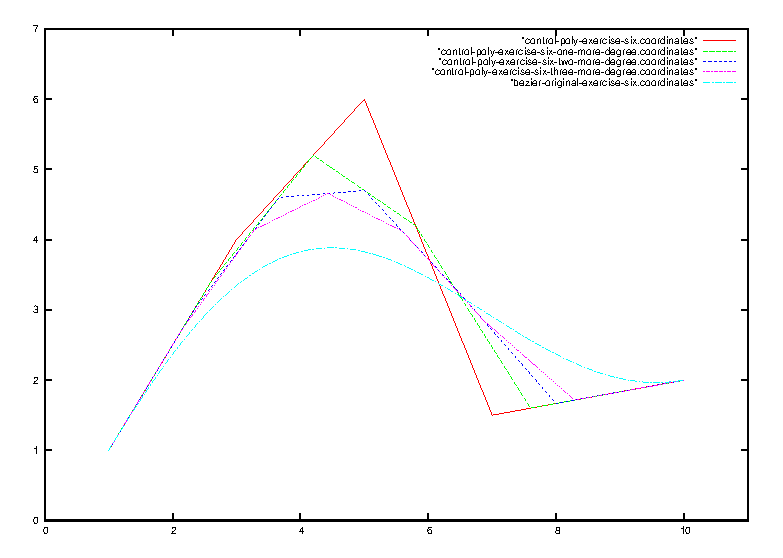
\includegraphics{bezier-deCasteljau-curves/exercise-six-higher-degree-control-poly}
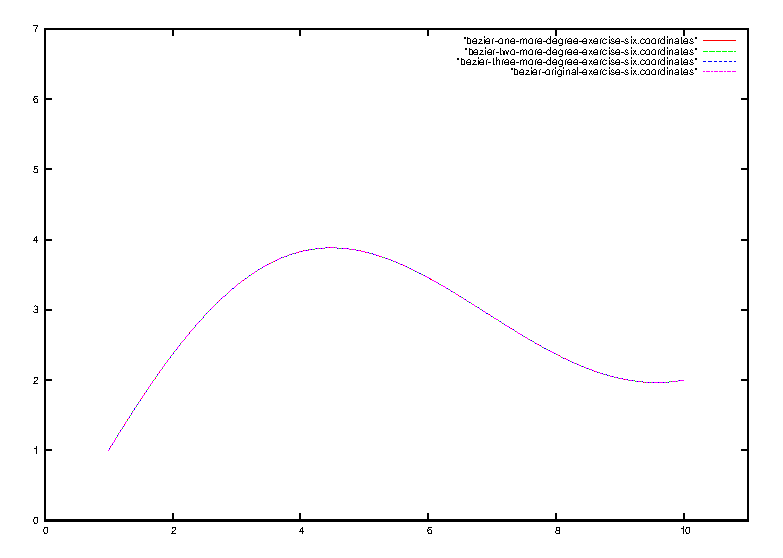
\includegraphics{bezier-deCasteljau-curves/exercise-six-one-more-degree-comparison}
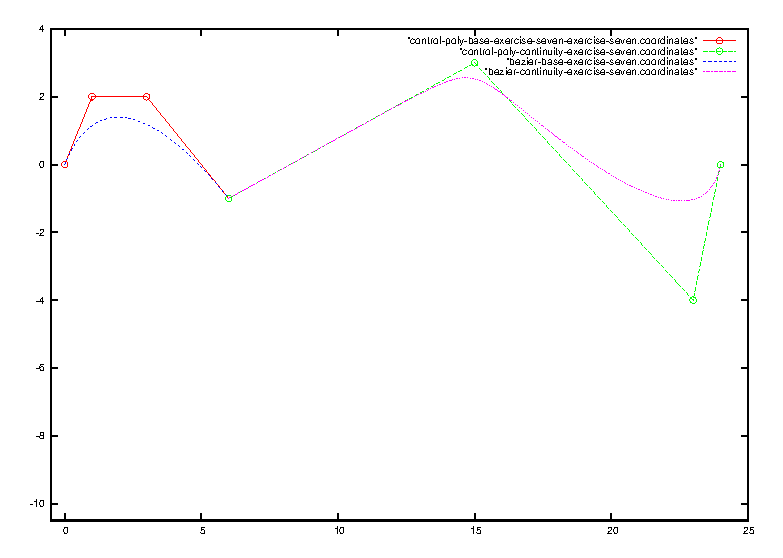
\includegraphics{bezier-deCasteljau-curves/exercise-seven-continuity}
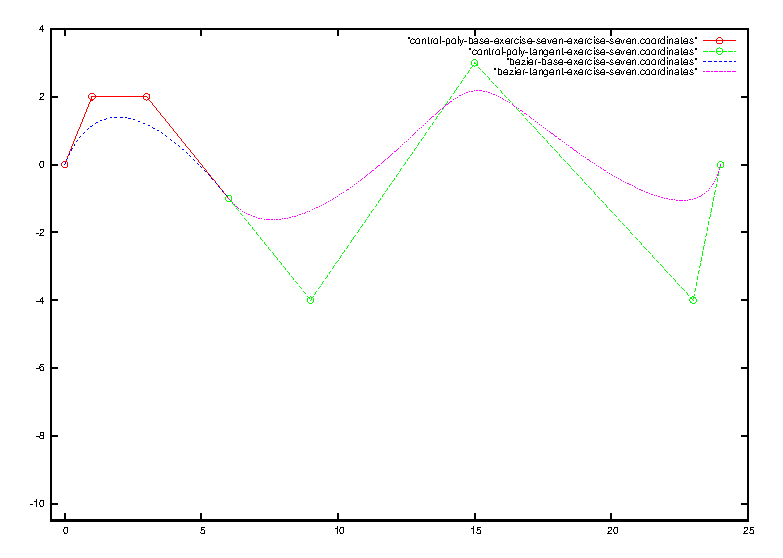
\includegraphics{bezier-deCasteljau-curves/exercise-seven-tangent}
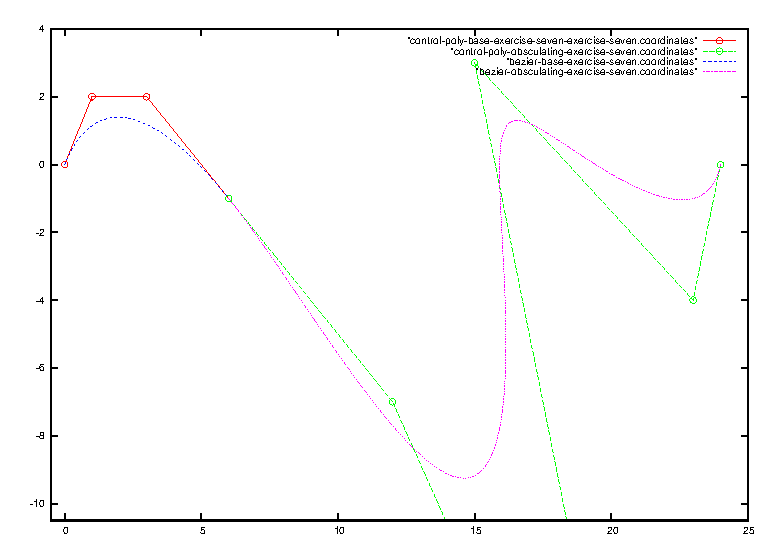
\includegraphics{bezier-deCasteljau-curves/exercise-seven-obsculating}
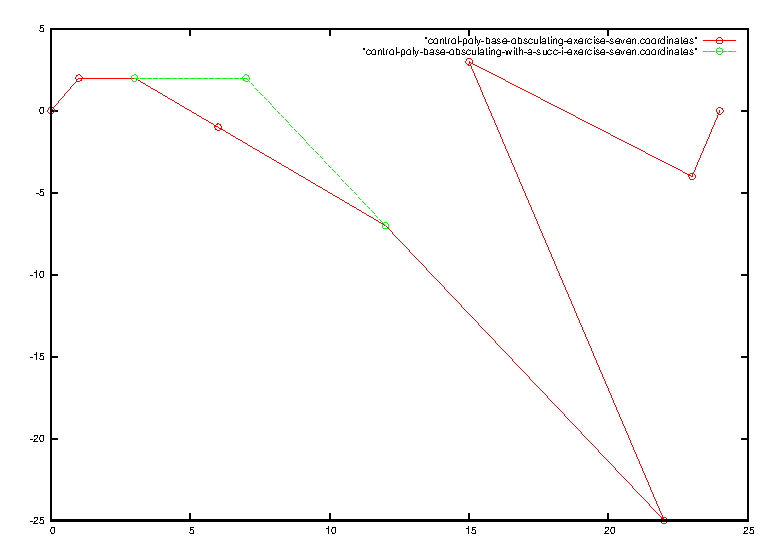
\includegraphics{bezier-deCasteljau-curves/exercise-seven-a_succ_i}
\includegraphics{bezier-deCasteljau-curves/exercise-seven-continuity-left}
\includegraphics{bezier-deCasteljau-curves/exercise-seven-tangent-left}
\includegraphics{bezier-deCasteljau-curves/exercise-seven-obsculating-left}
\includegraphics{bezier-deCasteljau-curves/exercise-seven-a_i-left}

\section{Code}
\verbatiminput{bezier-deCasteljau-curves/deCasteljau.jl}

\newpage

\begin{thebibliography}{}

\bibitem{FLP} Fischer M. J., Lynch N. A., Paterson M. S.,
  \emph{Impossibility of Distributed Consensus with One Faulty
    Process}, in "Journal of the Association for Computing Machinery",
  Vol. 32, No. 2, Aprile 1985, pp. 374-382.

\bibitem{ETH} Locher T., Y. A. Pignolet, R. Wattenhofer,
  \textit{Principles of Distribuited Computing}, Zurich, Swiss Federal
  Institute of Technology, 2013.


\end{thebibliography}



\end{document}
